\section{Theory and Engineering practices}
In this chapter is a list of the theories and engineering practises that where used during the course of the project. The first section of the chapter is the list of literature from which theories and practices where picked from. The second section is an overview of what the theories and practices where picked in the pre-study.  
\subsection{Literature study}
In the listing below is the literature used for getting the project started as well as used through out the project. It was used as source for gaining understanding of prevalent theories and practices for working in projects. The list includes project transcending sources that is applicable throughout the project. That means literature that all members of the group needs to have read. 

In the second section of the listing is role specific literature. This is literature the person having been assigned the role has to have good insight and understanding of. Meaning the person with the role has to understand the methods and theories presented in literature. However, it does not exclude the other members that also needs some, although limited, knowledge of the theories and methods of the same literature. This is has been important to facilitate communication. The knowledge have been conveyed by other members learning from the person having the role associated with that knowledge or by reading the literature themselves.            

\vspace{5mm} %5mm vertical space

\textbf{Project transcending sources}
\begin{itemize}
    \item Project health and status
        \begin{itemize}
            \item Alpha State Card Reference Guide \cite{noauthor_alpha_2015} 
        \end{itemize}
    \item Scrum
        \begin{itemize}
            \item Scrum and XP from the Trenches\cite{kniberg_scrum_2015}
        \end{itemize}
    \item Project phase division
        \begin{itemize}
            \item Essential Unified Process \cite{noauthor_essential_2016}
        \end{itemize}
    \item Project basics
        \begin{itemize}
            \item Chapter 1-3 Software Engineering \cite{ian_sommerville_software_nodate}
        \end{itemize}
    \item Person- and group dynamics
        \begin{itemize}
            \item Arbeta i projekt-individen, gruppen, ledaren \cite{eklund_arbeta_2010}
        \end{itemize}
\end{itemize}

\vspace{5mm} %5mm vertical space

\textbf{Project Management}
\begin{itemize}
    \item Chapter 22-23, 26 Software Development \cite{ian_sommerville_software_nodate} 
    \item Kanban - A brief introduction \cite{atlassian_kanban_nodate}
    \item Scrum - what it is, how it works, and why it's awesome \cite{atlassian_scrum_nodate}
    \item Role: Project Management Seminar slides \cite{lundevall_rollen_nodate}
\end{itemize}

\textbf{Customer \& Requirement}
\begin{itemize}
    \item Chapter 4 Software Development \cite{ian_sommerville_software_nodate}
    \item Role: Customer \& Requirement Seminar slides
    \begin{itemize}
        \item "Stories
        \item "UseCase"
    \end{itemize}
\end{itemize}

\textbf{Architecture}
\begin{itemize}
    \item Chapter 5-6 Software Development \cite{ian_sommerville_software_nodate}
    \item Role: Architect Seminar slides  \cite{tanyingyong_roll_nodate}
    \item Fundamentals of Software Architecture \cite{richards_fundamentals_2020}
    \item The C4 model for visualising software architecture \cite{brown_c4_nodate}
    \item The 4+1 View Model of Software Architecture \cite{kruchten_architectural_nodate}
\end{itemize}

\textbf{Development}
\begin{itemize}
    \item Chapter 7, 17, 25 Software Development \cite{ian_sommerville_software_nodate}
    \item Role: Development Seminar slides
\end{itemize}

\textbf{Testing} -
\begin{itemize}
    \item Chapter 8 Software Development \cite{ian_sommerville_software_nodate}
    \item Role: Testing Seminar slides  
    \item Test och kvalitetssäkring av IT-system \cite{eriksson_test_2008}
    \item A First Course in Object Oriented Development A Hands-On Approach \cite{lindback_first_2022}
    \item JavaScript End to End Testing Framework \cite{noauthor_javascript_nodate}
    \item Introduction to software testing concepts - Learn \cite{kendrahavens_introduction_nodate}
    \item Integration Testing: What is, Types, Top Down & Bottom Up Example \cite{hamilton_integration_2020}
    \item How to Write Test Cases: Sample Template with Examples \cite{hamilton_how_2020}
    \item Writing Your First Test \cite{noauthor_writing_nodate}
\end{itemize}

\textit{\textbf{Sustainability}}
\begin{itemize}
    \item Role: Sustainability Seminar slides  \cite{lundevall_rollen_nodate}
    \item Handbook of Usability Testing: How to Plan, Design, and Conduct Effective Tests \cite{rubin_handbook_2011}
    \item Arbetsmiljön är viktig \cite{noauthor_arbetsmiljon_nodate}
    \item Perspectives on GDPR - The GDPR for  Operations - What Should Software Engineers Know About the GDPR? \cite{pais_perspectives_nodate}

\end{itemize}

\subsection{Pre-study}
Due to limited experience in project work the students where given a proposition for an approach of project method by the examiner of the course. This was done by referring to the online book ”Scrum and XP from the Trenches” \cite{kniberg_scrum_2015} which was studied to get an understanding of the Scrum methodology. For the role-playing aspects of the project some references on Canvas prompted reading sections of the book "Software Engineering" \cite{ian_sommerville_software_nodate} to give an overview of the requirements for each role. 

This meant the adoption of a strict Scrum methodology for the first iteration described in ”Scrum and XP from the Trenches”  \cite{kniberg_scrum_2015} As the project progressed elements of the Scrum methodology was modified throughout the following iteration. For example, the daily scrum went from being a daily activity to only be held on days where the project group got together. Other methods from Scrum that were tested were: digital and physical product and sprint backlog, digital and physical task board, story points, iteration planning, retrospective, and burndown chart. The reason for the backlogs and the task boards being both digital and physical was that it made it possible to efficiently work remotely if needed. The physical was used only for planning.

Apart from the methodology derived from Scrum some other methods and techniques were used. Meetings agendas to handle decision-making were created and used. Prioritization using MoSCoW analysis was used for deriving product functionality was another technique implemented during the project. As part of the role-playing dimension for the project architecture, testing, development, and vision documents where created including models.

\begin{enumerate}
    \item \textit{Arbetstavla}
    \begin{figure}[htbp]
        \centerline{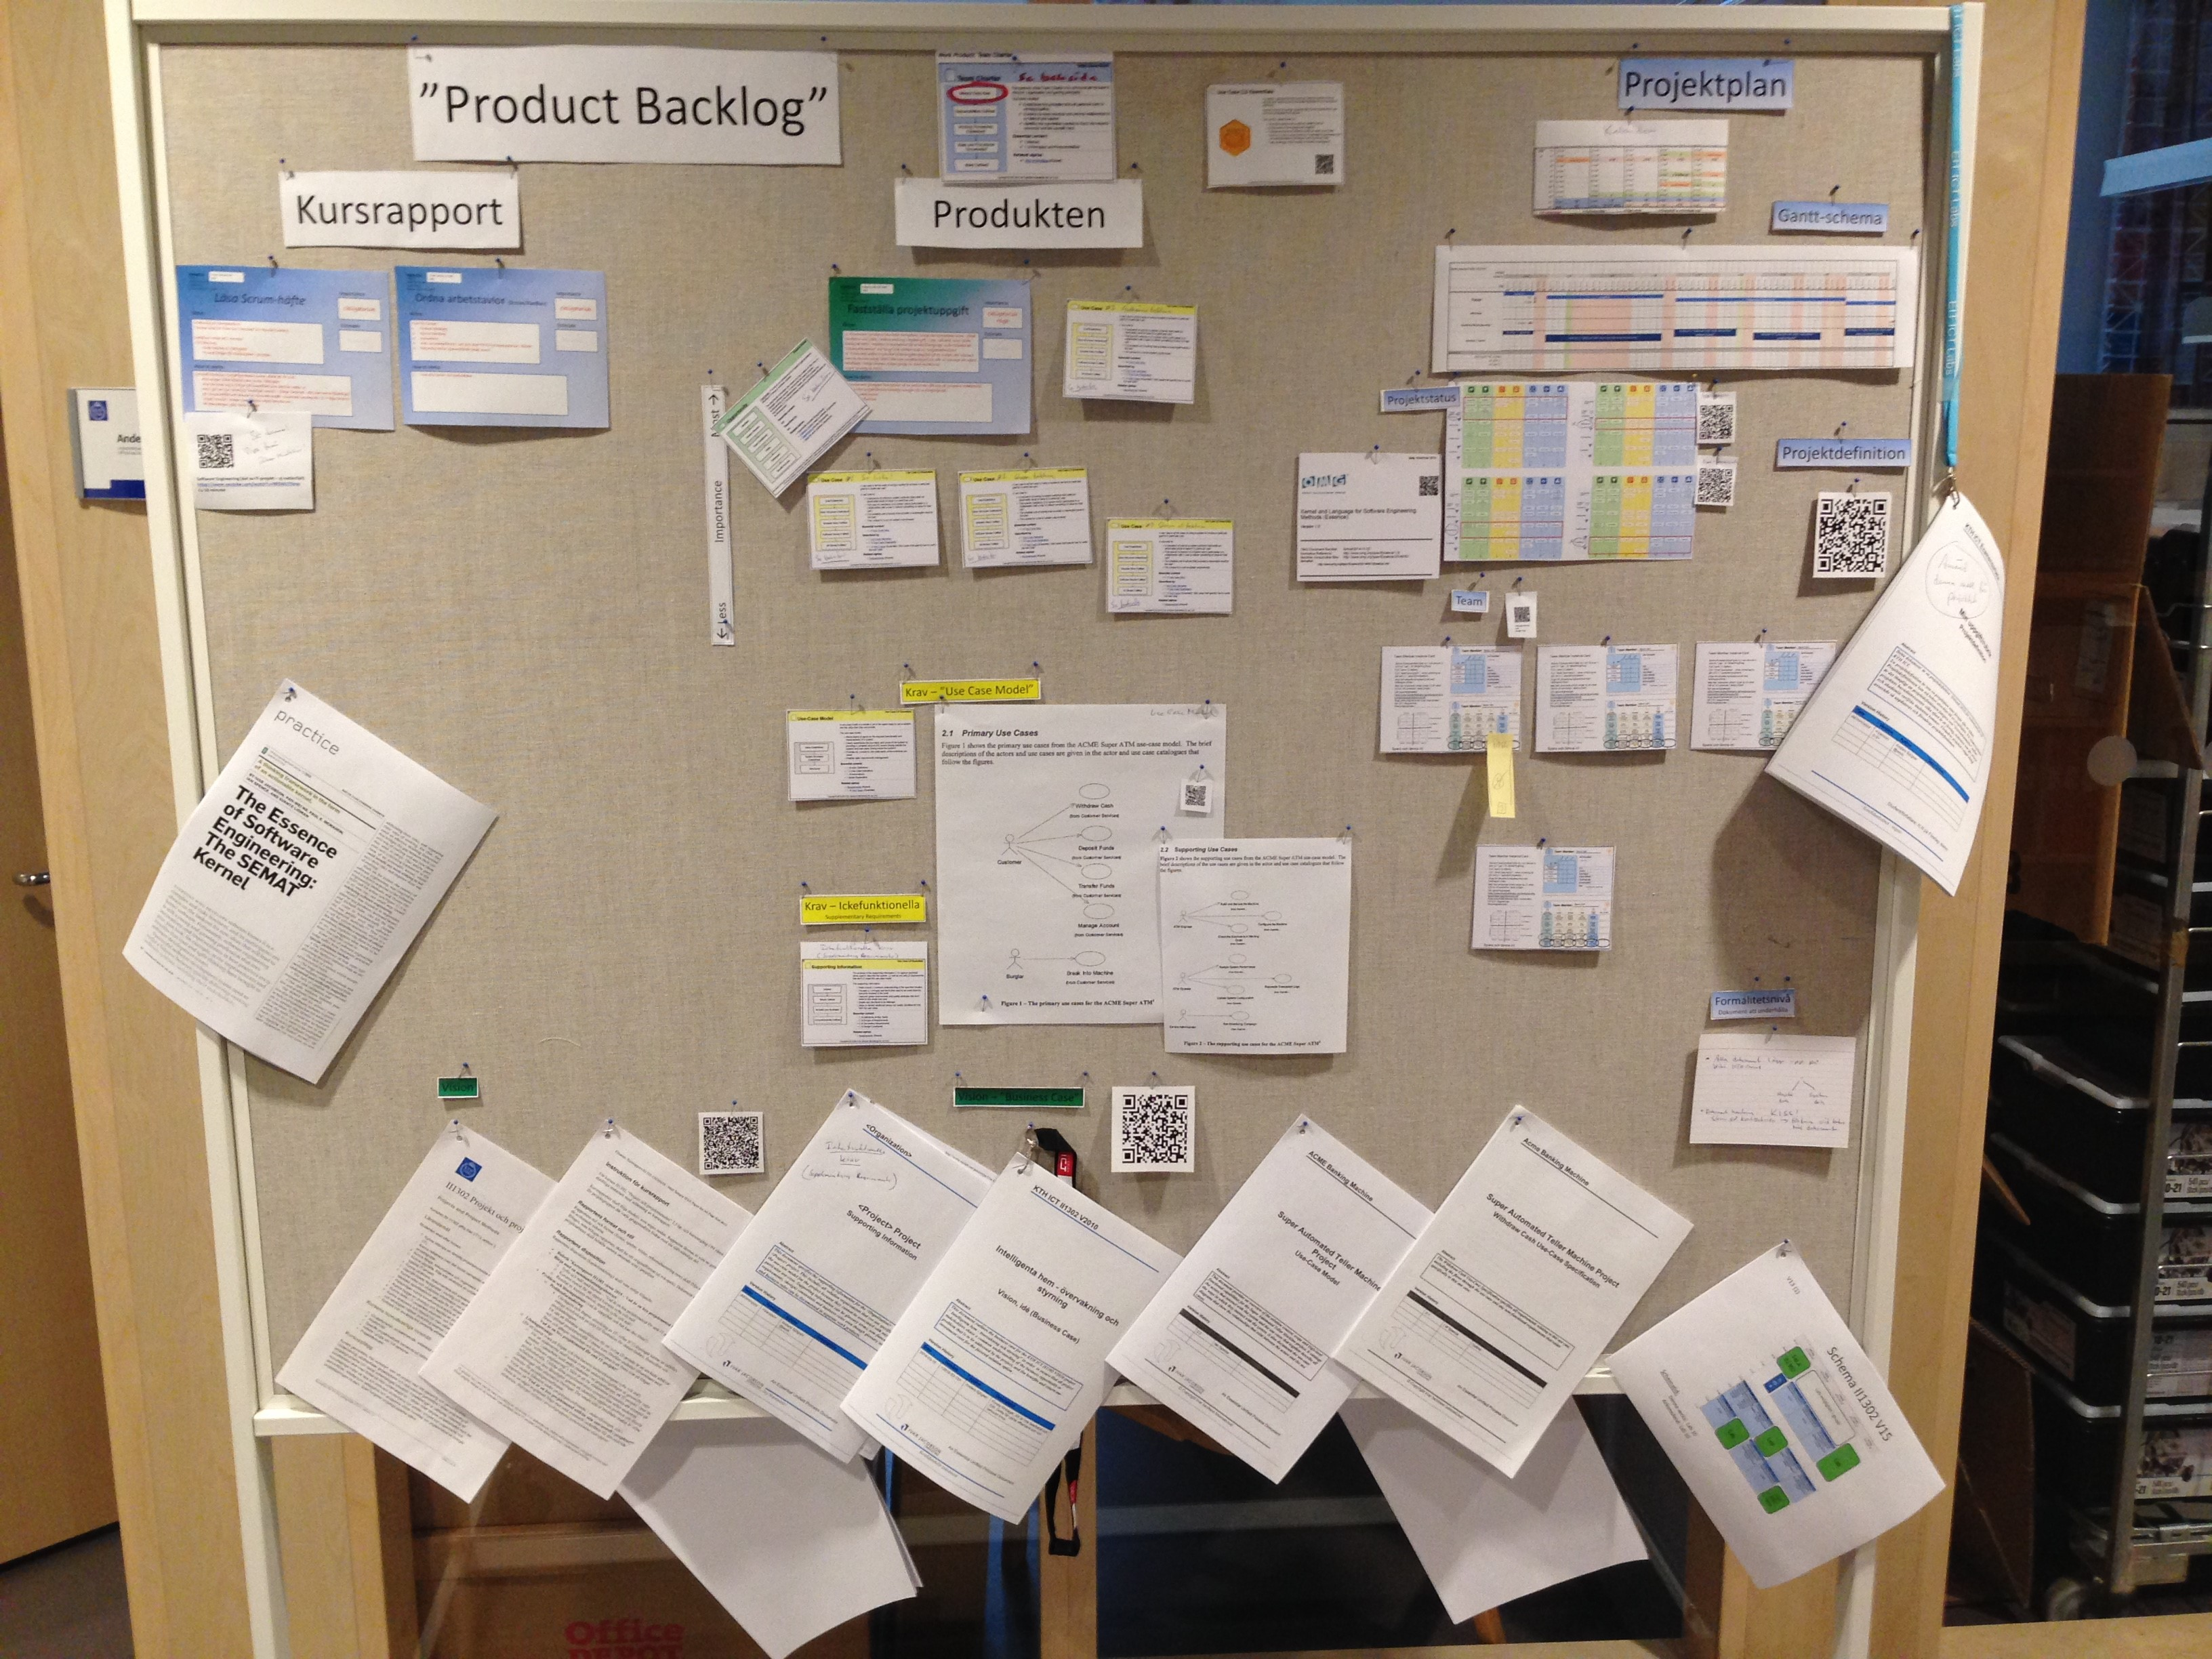
\includegraphics[max height=250px, max width=250px]{Z. images/arbetstavla.jpg}}
        \caption{Arbetstavla "nåldyna"}
        \label{fig}
    \end{figure}
    
    \begin{figure}[htbp]
        \centerline{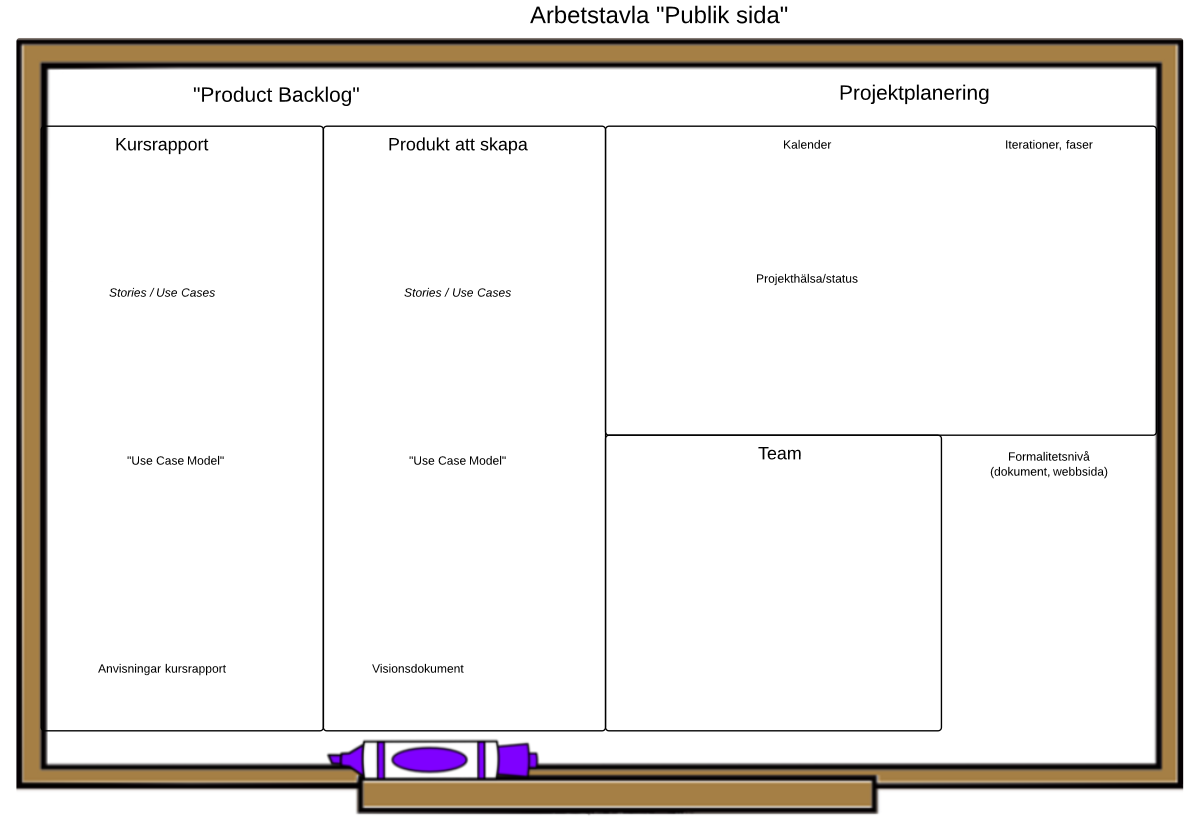
\includegraphics[max height=250px, max width=250px]{Z. images/lucidtavla.png}}
        \caption{Arbetstavla "whiteboard" "Publik sida"}
        \label{fig}
    \end{figure}

    \begin{figure}[htbp]
        \centerline{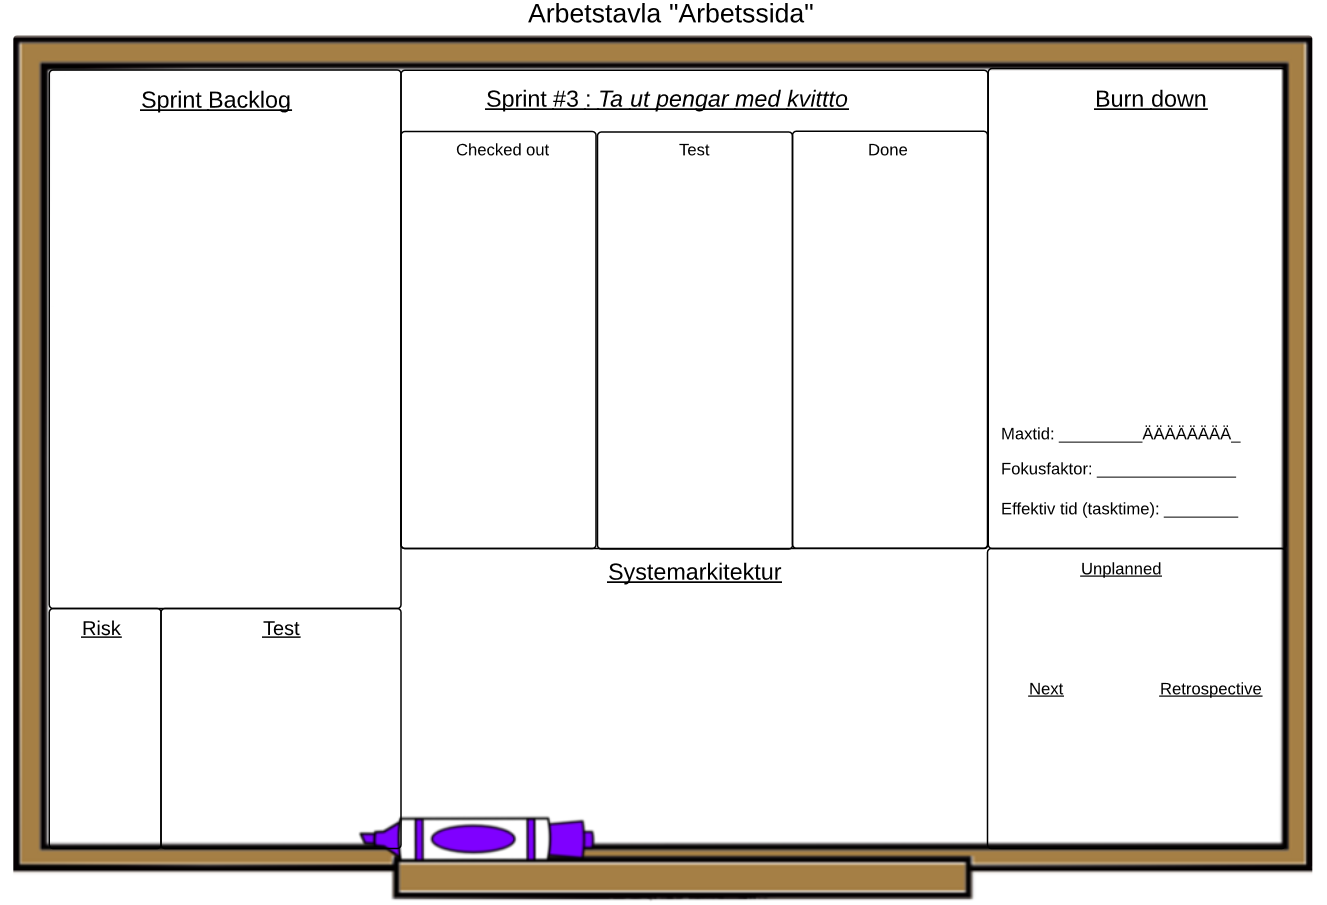
\includegraphics[max height=250px, max width=250px]{Z. images/lucidbaksida.png}}
        \caption{Arbetstavla "whiteboard" "Arbetssida"}
        \label{fig}
    \end{figure}
    \item \textit{Scruminspirerade projektaktiviteter}
    Bilden nedan visar projektmodellens aktiviteter och ordning.

    \begin{figure}[htbp]
        \centerline{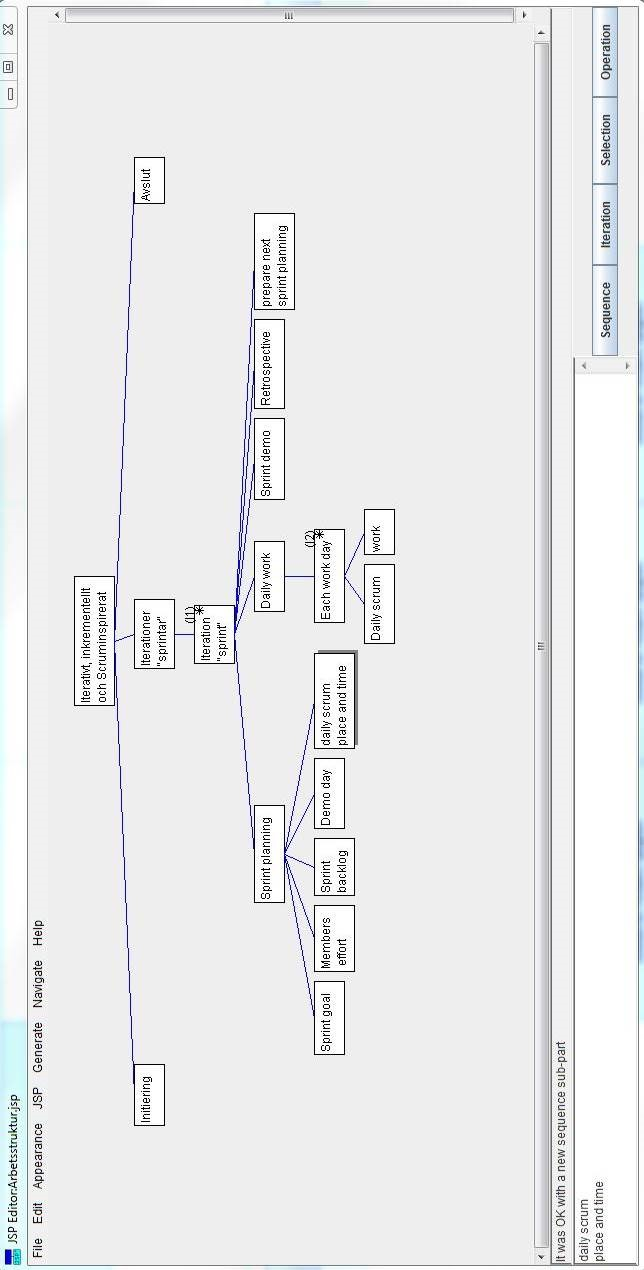
\includegraphics[max height=250px, max width=250px]{Z. images/scrum.jpg}}
        \caption{Den här har ingen beskrivning i mallen.}
        \label{fig}
    \end{figure}
\end{enumerate}